\chapter{Description \& Methodology}

\section{Convolution}
Some words on convolution. Background-ish

\section{FPGA}

The very heart of our computer is our custom made architecture implemented on our FPGA.
In this section we will first describe the overall architecture of our convolution engine, and then we will drill down and examine the core modules.
Modularity and extendibility is a core principle in our design, however in this section we will describe the processor as if only being able to do 3x3 convolutions.

\subsection{Overall design}

Convolution is a very regular task where data flows only forward. This means that our processor can be simplified, removing the need for a central control module.
Instead each module simply operates under the assumption that all data inputs are correctly formatted and ordered and does its operations accordingly.
\begin{figure}[h!]
    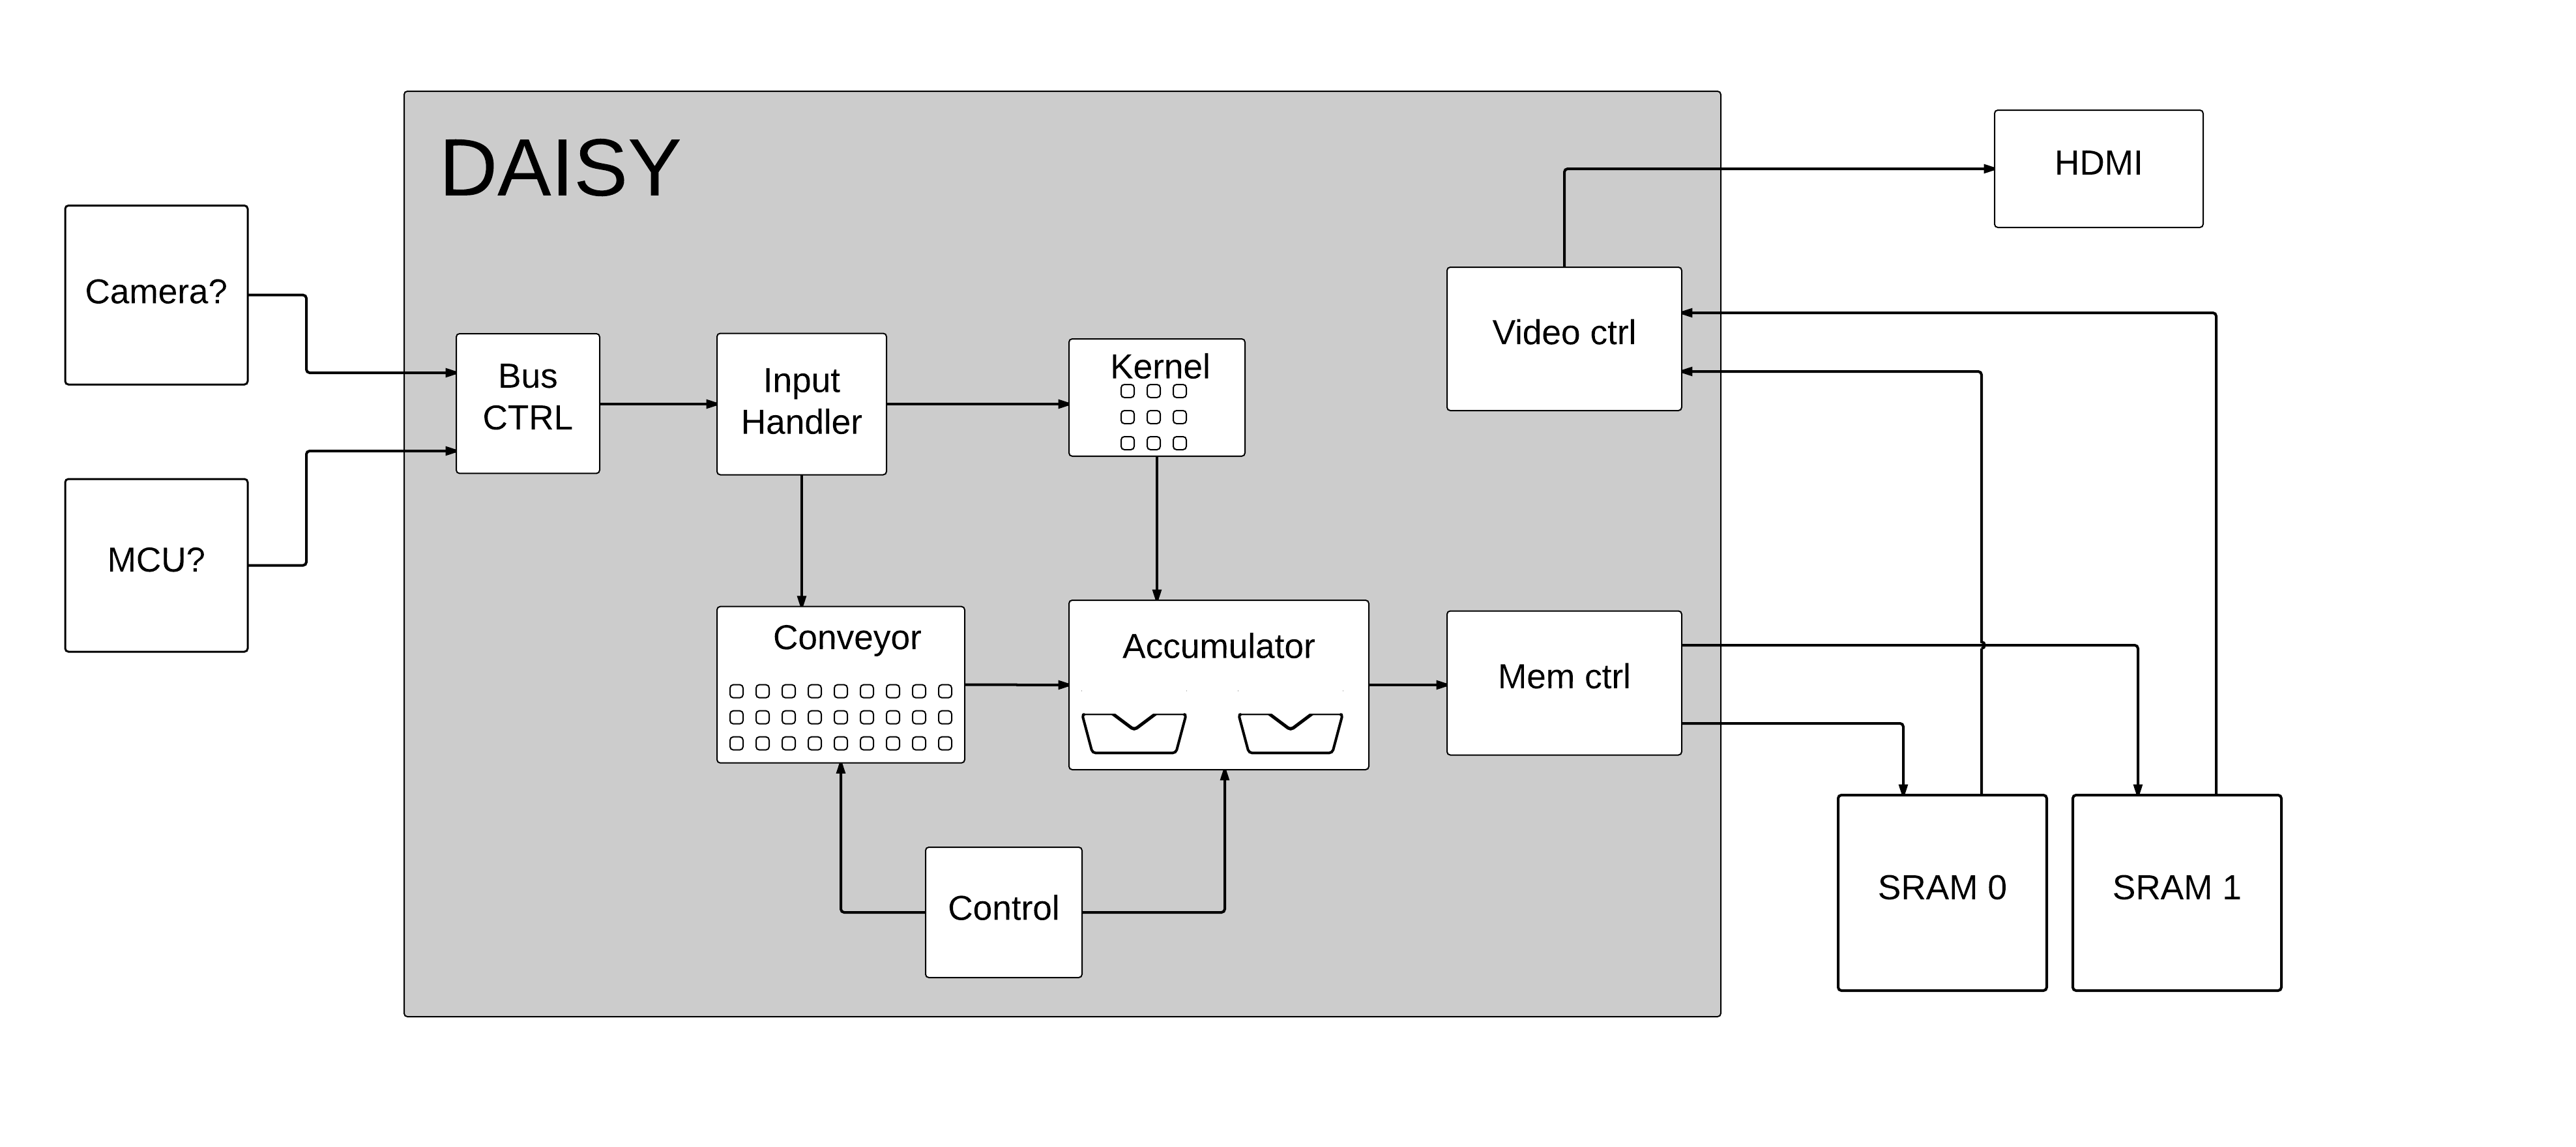
\includegraphics[width=\linewidth]{img/DataPath.png}
    \caption{The data path for our processor, named daisy after the way it daisy chains control}
    \label{fig:Convolution}
\end{figure}
In the figure we see this design principle reflected, no data ever flows backwards, only forwards. 
Breaking up the individual steps we get the typical flow of data.
\begin{enumerate}
  \item Data from the bus is read by the bus controller. This controller serves as a clock domain crossover and is responsible for delivering data to the input handler in a clock domain crossing FIFO queue.
  \item The input handler recieves data from the queue and does magic
  \item After magic is performed the conveyor recieves the data. This unit is responsible for buffering pixel data, and deliver data to the accumulator in a set pattern to ensure a pixel is used in all its 9 contexts.
  \item The Kernel buffer collects kernel data at program start from the input handler. After recieving 9 kernel values it will only deliver kernel data to the Accumulator
  \item The accumulator recieves kernel data from the kernel buffer and performs its mapping function on the kernel value and the pixel from the conveyor belt. 
When an accumulator has accumulated all its pixels it flushes its value, resetting the accumulator register and writing the old data to the memory control unit.
  \item Accumulated pixels are reassembled in the mem ctrl unit and written to one of the two SRAM banks, allowing us to double buffer. 
  \item After being buffered in SRAM pixel data is read by the video ctrl module which outputs video to an HDMI cable, ensuring crisp image quality served in a modern fashion.
\end{enumerate}

\section{Data in}

We used an EBI bus!
We handled data in an input buffer!

\section{Convolver}
This section encompasses the four modules forming the heart of the convolution engine. In the order they are covered, they are:
\begin{enumerate}
    \item the conveyor belt 
    \item the kernel buffer 
    \item the accumulator.
    \item the control unit
\end{enumerate}
In order to not bog down the report with unescessary implementation detail we will cover an idealized implementation leaving the final implementation to the appendix.
The two major parts of the convolution engine is the conveyor belt and the accumultion unit. By decoupling these we ensure a modular design allowing us to try a range of different approaches in our accumultion unit.

\subsection{The conveyor belt}
In order to convolute an image we make several sweeps over the image as shown in fig:Sweeps. 
fig:SweepFrontier shows the frontier of each sweep, highlighting the three rows currently residing in the conveyor.
\begin{figure}[h!]
    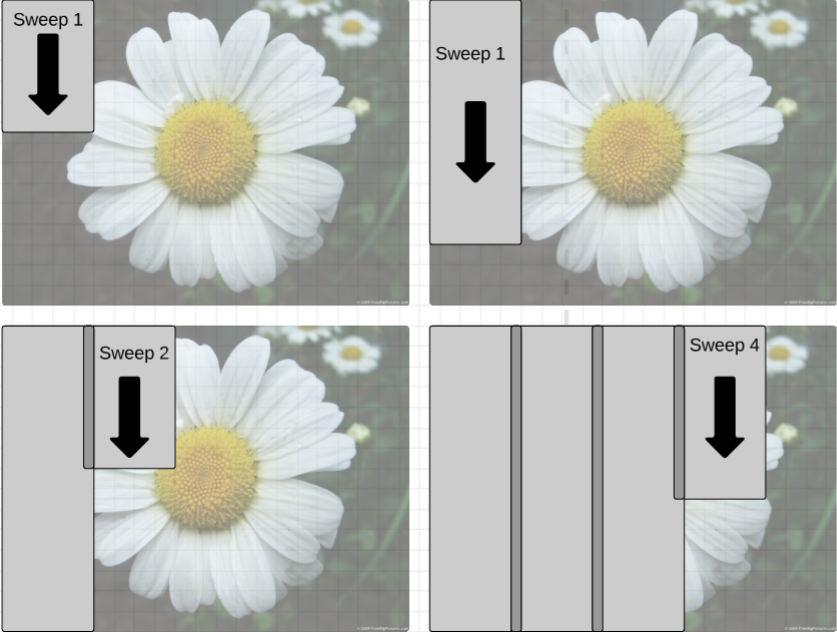
\includegraphics[width=\linewidth]{img/Sweeps.png}
    \caption{The sweep pattern used to collect data for convolution}
    \label{fig:Sweeps}
\end{figure}
\begin{figure}[h!]
    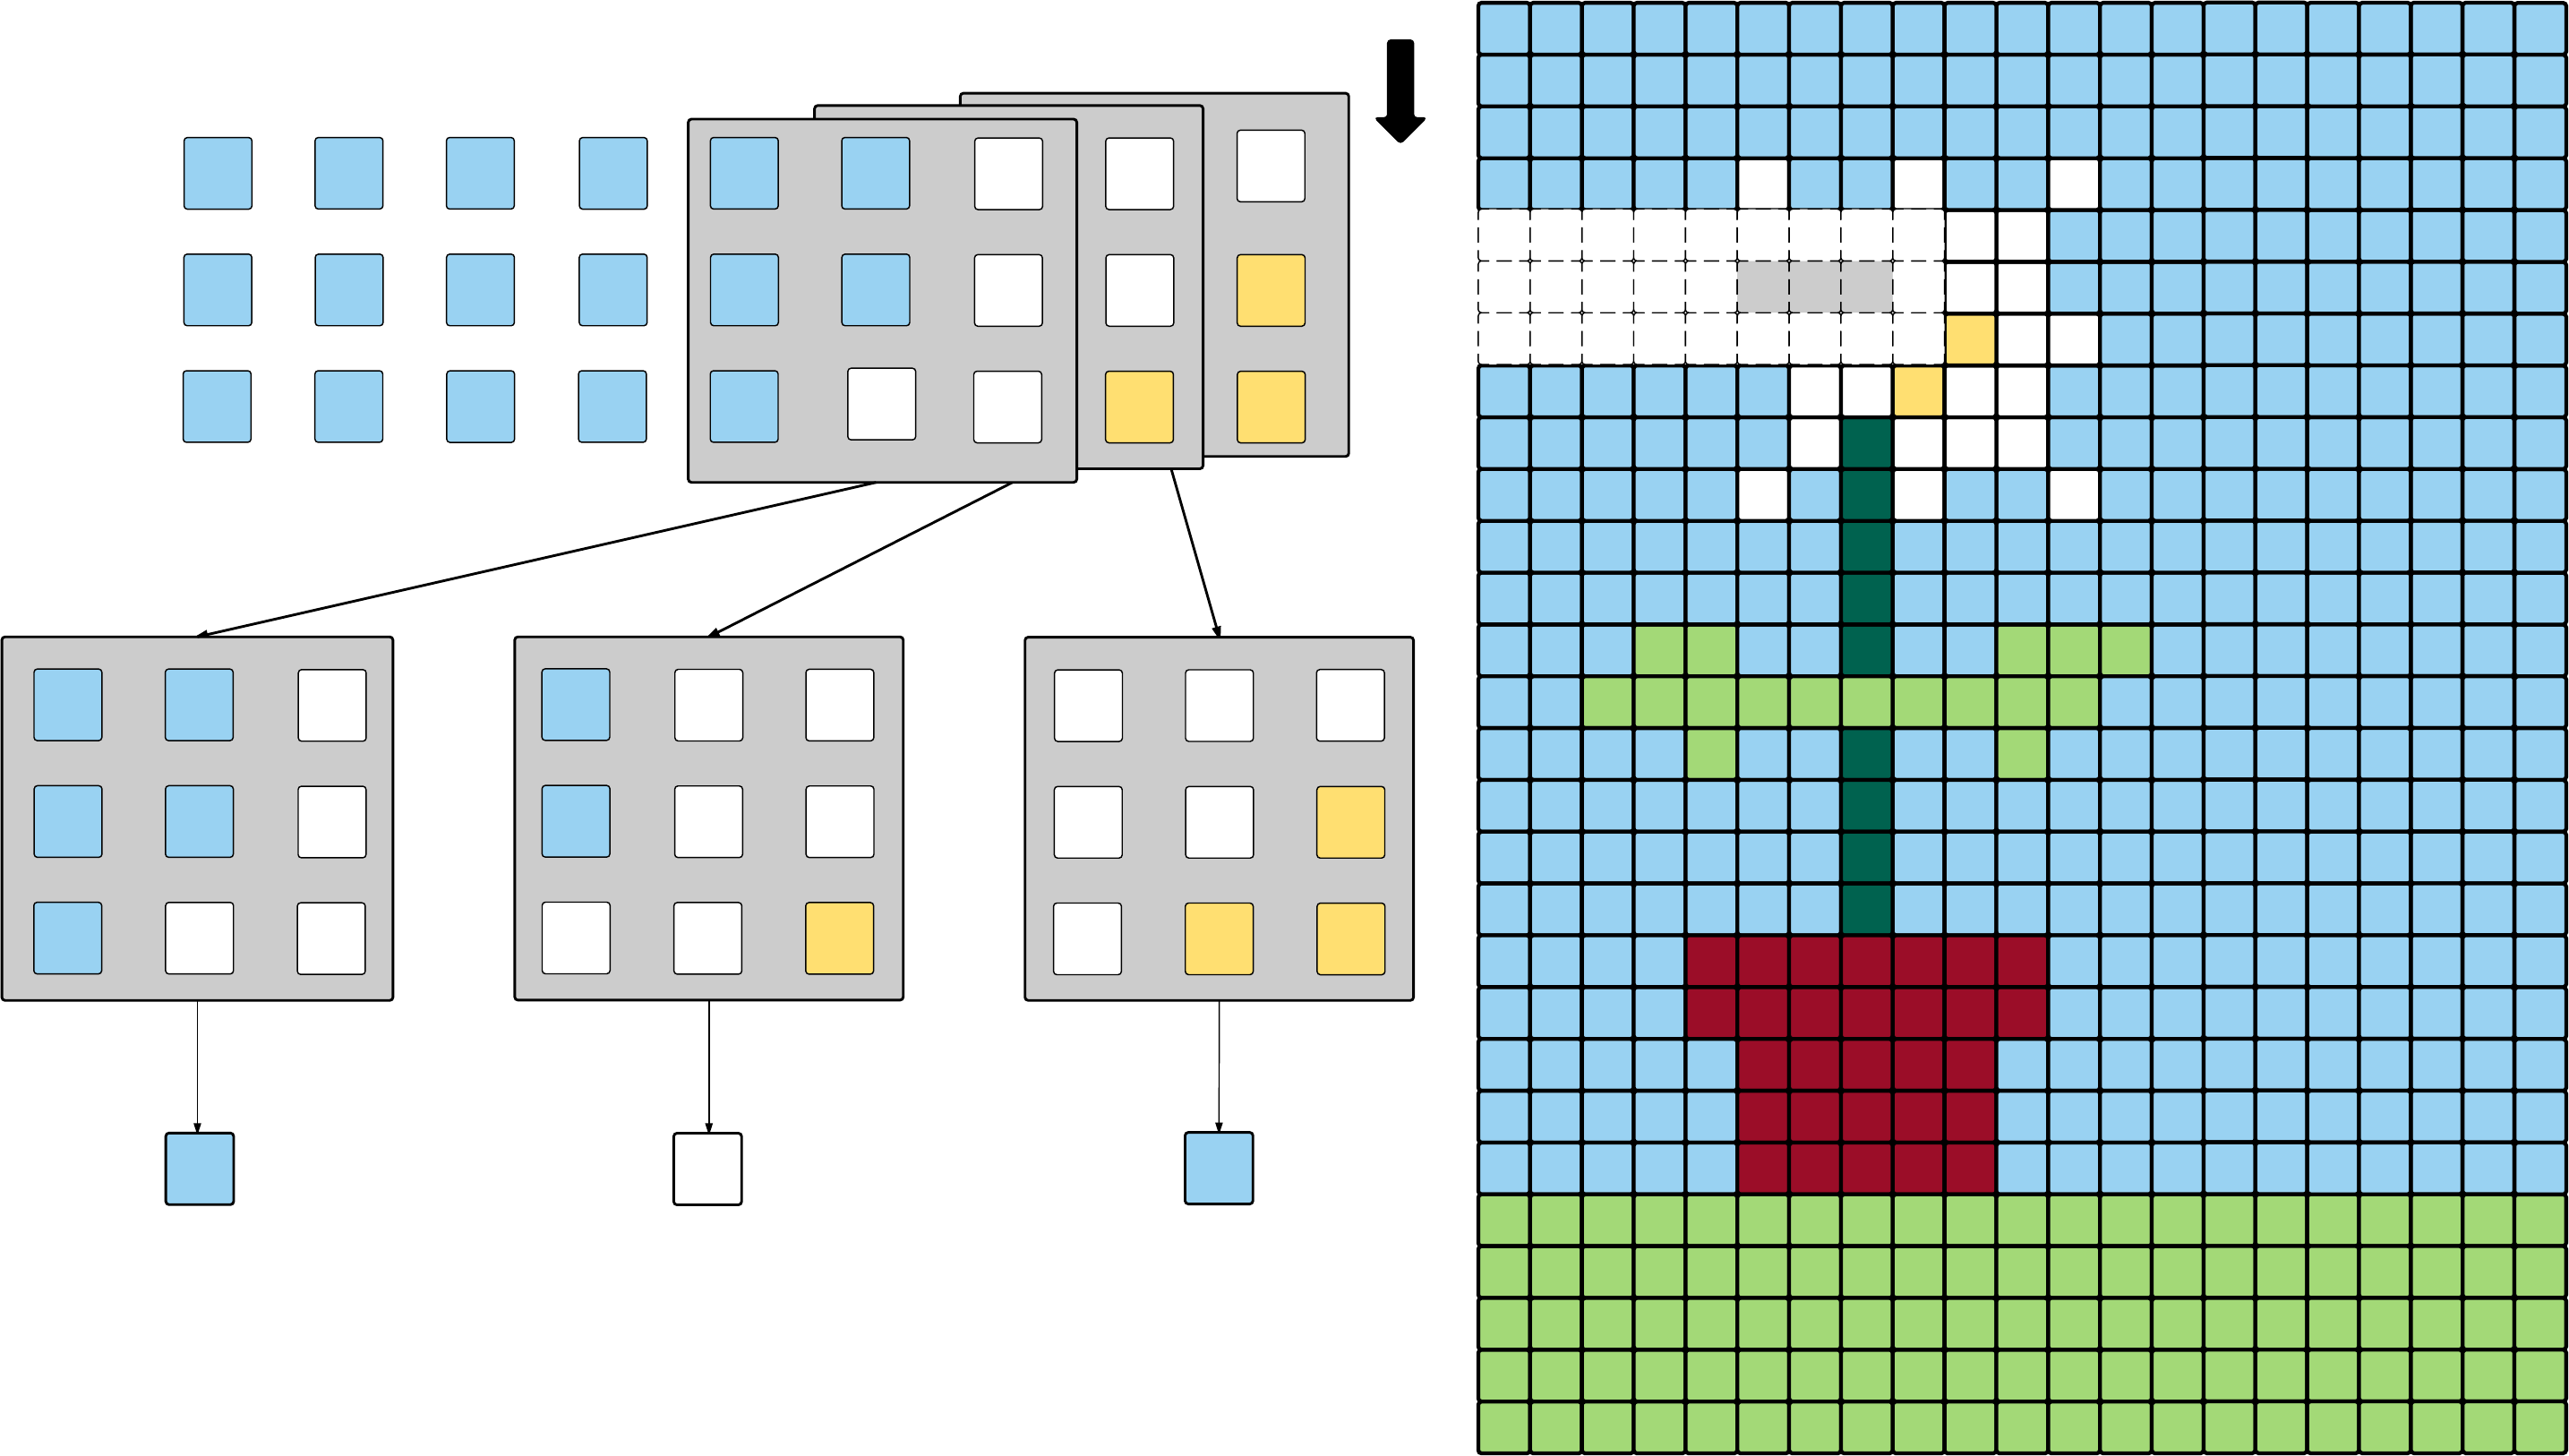
\includegraphics[width=\linewidth]{img/FeedPattern.png}
    \caption{The image three greyed out pixels in the source image represent the three pixels which the neighbourhoods in grey boxes help calculate. The window is three pixels deep and nine pixels wide}
    \label{fig:SweepFrontier}
\end{figure}
The job of the conveyor belt is to maintain the convolution frontier and to feed the accumulators with data. An ideal representation of the conveyor belt is shown in fig:Ideal
\begin{figure}[h!]
    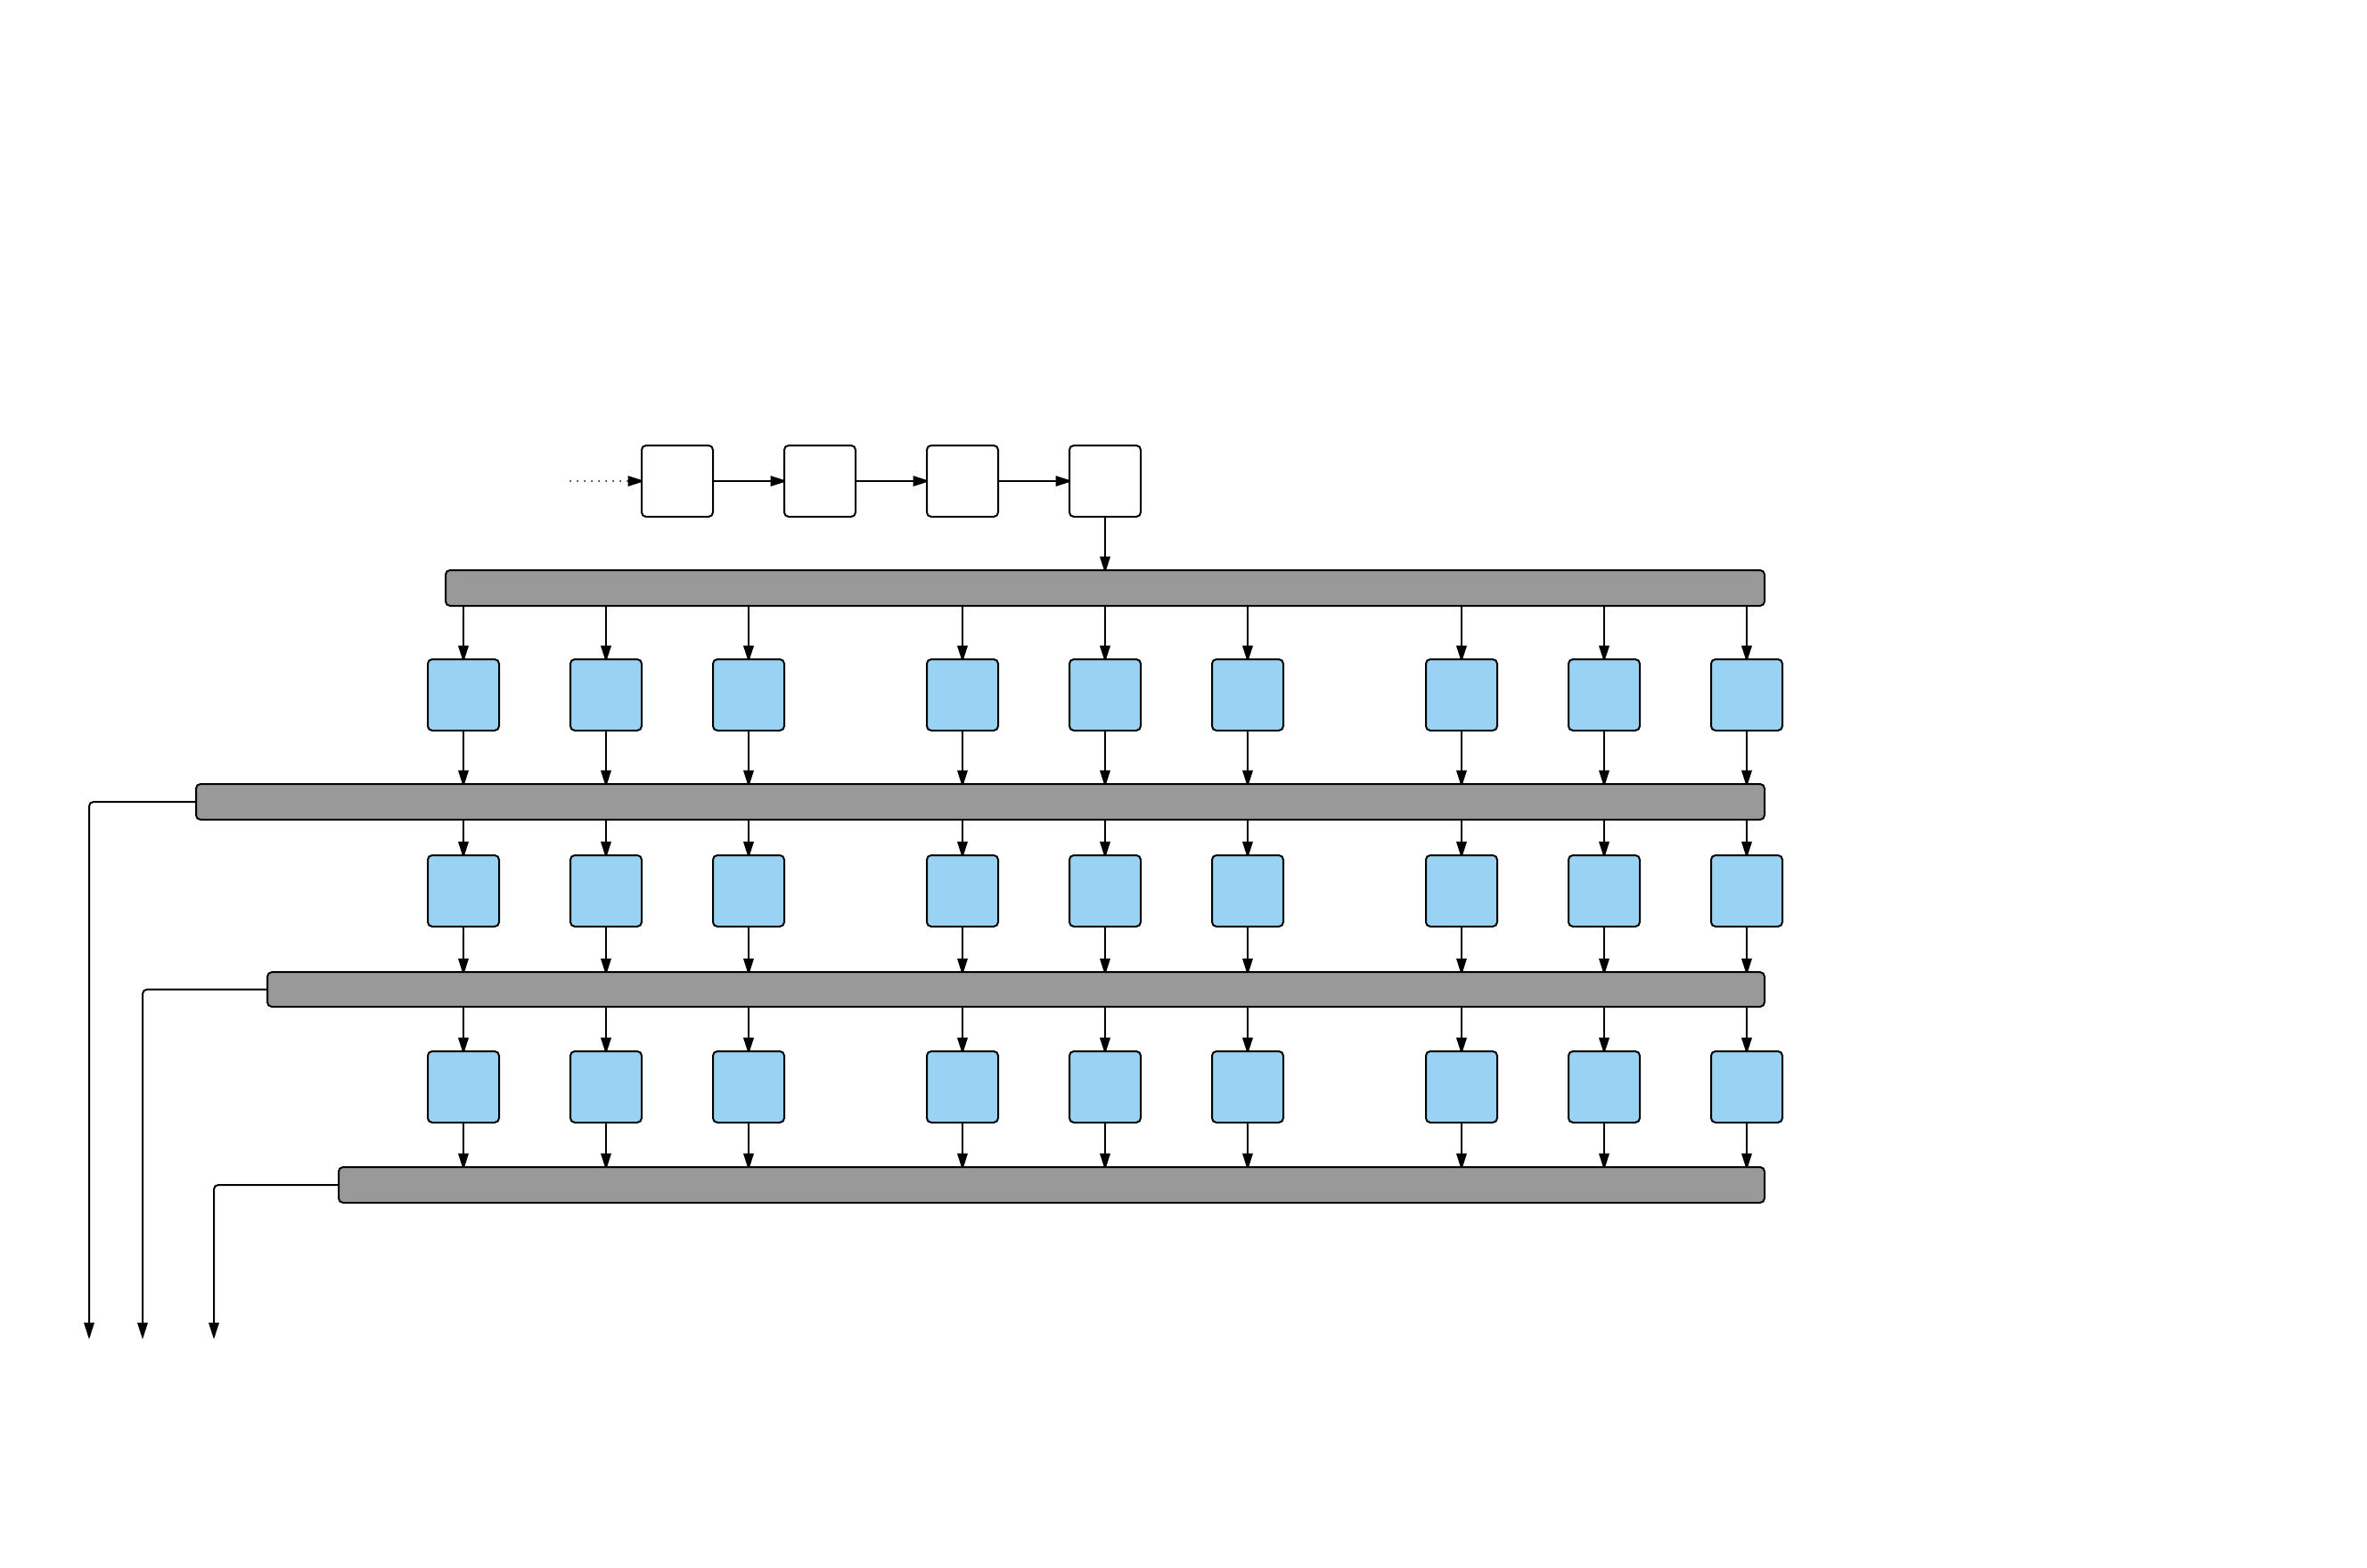
\includegraphics[width=\linewidth]{img/IdealFeeder.png}
    \caption{TODO}
    \label{fig:Contexts}
\end{figure}
